\chapter{視界、狀態方程與真空能}

\section{優選參考系、超光速退行與視界}

宇宙微波背景輻射確實標示出一個特殊參考系。在這個參考系中，該輻射看起來是各向同性的；附近星系平均而言也處於靜止。如果我們相對於背景運動，前進方向上的光子會因多普勒效應而移向較高能量，後退方向上的光子則移向較低能量。優選參考系就是微波背景看起來各向同性的參考系；平均而言，本地星系也在這個參考系中靜止。

\begin{classroomqa}
\lecturetimestamp{00:00:25}
\audiencequestion{宇宙輻射的表觀波長是否取決於觀測者的運動？這是否意味著存在優選參考系？}
\lecturerresponse{是的。相對於微波背景運動會產生多普勒各向異性，因此存在一個優選的宇宙學參考系，也就是微波背景看起來各向同性的參考系。平均而言，本地星系也在這個參考系中靜止。}
\end{classroomqa}

第二個問題關於退行速度。哈伯定律指出，足夠遙遠的星系彼此遠離的速度符合
\begin{equation}
v = H d .
\end{equation}
當 \(d\) 夠大時，這個退行速度會超過光速。這並不違反相對論，因為相對論的限制是局部的：一個物體不能在我們眼前以超光速掠過另一個物體。遙遠星系的情形，描述的是相距甚遠的地方之間的幾何關係。

\begin{classroomqa}
\lecturetimestamp{00:04:48}
\audiencequestion{兩個星系的相對速度能否大於 \(c\)？}
\lecturerresponse{可以，只要它們相距夠遠。哈伯退行速度可以超過光速而不違反局部相對論；退行速度達到 \(c\) 的地方就是視界。}
\end{classroomqa}

退行速度一旦達到光速，朝我們傳來的訊號就不再能縮短與我們之間的距離。光線在局部仍以極限速度前進，但它必須追上的距離增長得太快。

\begin{classroomqa}
\lecturetimestamp{00:07:03}
\audiencequestion{反方向發出的光線，難道不還是會朝我們前進嗎？}
\lecturerresponse{在局部確實如此，但空間膨脹的速度超過了光線追上我們的速度。光線相對於附近位置以極限速度前進，但回到我們這裡的總距離仍持續增加。}
\end{classroomqa}

\section{膨脹度規與直線類比}

一個有用的圖像是一維直線。想像一條由原子構成的線。若拉伸一條普通材料線，它最後會斷裂。現在改變這個圖像：每當相鄰原子相距太遠，就在它們之間插入另一個原子。這條線持續變長，但其局部性質不會因此變得稀疏。

\begin{figure}
\centering
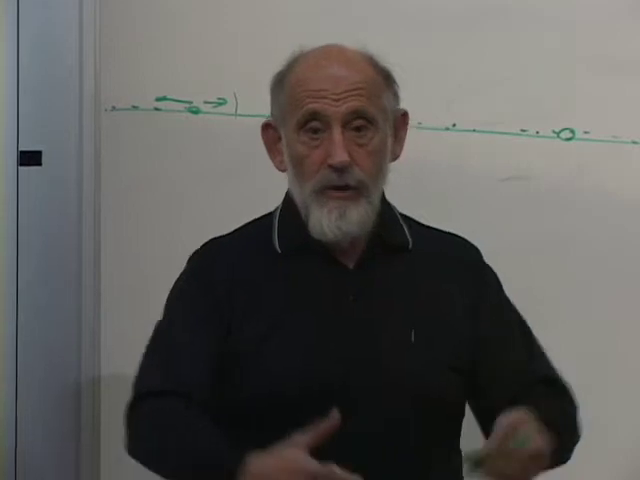
\includegraphics[width=0.60\textwidth]{lecture_04_figure_02.png}
\caption{用來描繪膨脹度規的一維直線。}
\end{figure}

在這個圖像中，局部仍有一個訊號速度上限，就像普通直線上的聲音也有速度上限。這條規則適用於局部：相對於附近的位置，擾動不能超過該速度。然而，如果直線夠長，而且新位置插入得夠快，距離夠遠的部分就會退行得太快，使訊號永遠無法返回。

因此，狹義相對論的速度合成定律只說明了部分情況。它適用於局部，也就是觀測者在同一位置彼此經過時。對於膨脹幾何中相距遙遠的星系，這並不是合適的描述方式。

\begin{classroomqa}
\lecturetimestamp{00:09:42}
\audiencequestion{在這種情況下，通常的相對論速度合成定律仍然適用嗎？}
\lecturerresponse{在局部、同一位置上，適用。如果觀測者依序彼此經過，通常的狹義相對論規則就適用。但要描述相距遙遠、退行速度超過 \(c\) 的情況，就不能用這種方式；必須回到膨脹空間的幾何。}
\end{classroomqa}

同一個圖像也能簡單說明紅移。在直線上畫一道波。直線膨脹時，波長也隨之伸長。在膨脹幾何中，這不只是形象化的說法；膨脹時空中的波動方程確實會導出波長伸長。

\begin{classroomqa}
\lecturetimestamp{00:14:42}
\audiencequestion{波隨著宇宙膨脹而伸長，這是理論推論、觀測結果，還是兩者皆是？}
\lecturerresponse{這是波在膨脹時空中傳播的理論推論，也有天文觀測支持。}
\end{classroomqa}

這個圖像不是橡皮筋。橡皮筋拉伸時會變細；生活在這種介質中的人會觀察到局部性質改變。這裡的局部性質保持不變，增長的是整體距離尺度。

\section{最後散射與可觀測宇宙}

視界是退行速度達到光速的地方。最後散射面位於視界稍內側。從視界發出的訊號會被無限紅移；最後散射輻射的紅移則極大，但仍有限。

\begin{classroomqa}
\lecturetimestamp{00:17:53}
\audiencequestion{超光速退行、最後散射面與可觀測宇宙之間有什麼關係？}
\lecturerresponse{視界是退行速度達到光速的地方。最後散射面位於視界稍內側，因為其紅移極大但仍有限。就實際而言，它標示了可觀測宇宙的邊界。}
\end{classroomqa}

最後散射輻射的紅移大約是 \(10^3\) 倍。這個數值已經非常大，因此在許多情況下，最後散射面都非常接近視界。可觀測宇宙是光能夠從中傳到我們這裡的那部分宇宙。

在晚期，膨脹會趨近真空能主導的狀態。此時哈伯參數趨於常數，視界則趨近固定大小；星系和微波輻射也會逐漸從視野中消失。

\begin{classroomqa}
\lecturetimestamp{00:22:43}
\audiencequestion{既然 \(H\) 會隨時間變化，視界距離也會變化嗎？微波背景最終會消失嗎？}
\lecturerresponse{在晚期，\(H\) 會趨於常數，因此視界會趨近固定距離。微波背景會持續伸長、冷卻並逐漸變得不可見。遙遠星系也會越過視界，從視野中消失。}
\end{classroomqa}

只有已受引力束縛的結構會繼續留在可觀測範圍內。太陽系不會飛散，星系也不會飛散，但大尺度宇宙會變成一座孤島。

\section{基本膨脹方程與三種組分}

現在來看基本膨脹方程：
\begin{equation}
\left(\frac{\dot a}{a}\right)^2 = \frac{8\pi G}{3}\rho ,
\qquad c=1 .
\end{equation}
其中 \(a(t)\) 是尺度因子，\(\rho\) 是總能量密度。

\begin{figure}
\centering
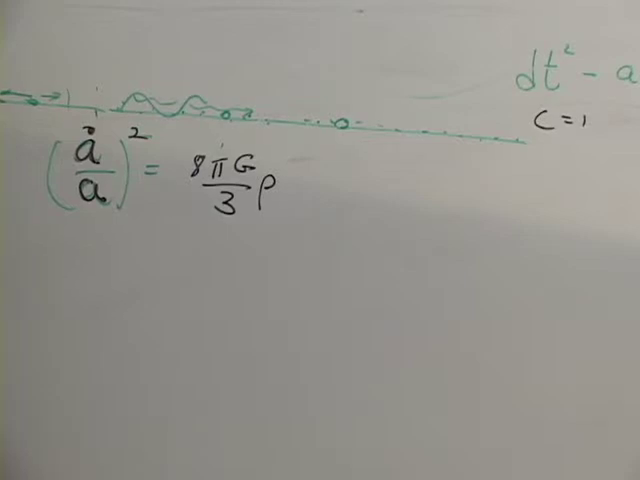
\includegraphics[width=0.74\textwidth]{lecture_04_figure_03.png}
\caption{基本膨脹方程與一維直線類比。}
\end{figure}

有三種組分在動力學上相當重要。

對物質而言，
\begin{equation}
\rho=\frac{\text{const.}}{a^3},
\qquad
a(t)\sim t^{2/3}.
\end{equation}
這描述有質量的物體隨整體膨脹運動，並且在共動參考系中基本上處於靜止的情況。

對輻射而言，
\begin{equation}
\rho=\frac{\text{const.}}{a^4},
\qquad
a(t)\sim t^{1/2}.
\end{equation}
多出的 \(a\) 次方來自宇宙膨脹時每個光子的紅移。

此外還有
\begin{equation}
\rho_0=\text{constant},
\end{equation}
真空能，也稱為暗能量；若不計傳統約定中的數值因子，它也稱為宇宙學常數。這種組分完全不會稀釋。

下一步是把能量密度和壓力聯繫起來。

\section{輻射壓力與冷物質}

先從輻射談起。考慮一個一維盒子，也就是長度為 \(L\) 的線段，裡面有光子來回反射。在一維中，力和壓力實際上是同一回事。

取一個動量大小為 \(p\) 的光子。它從盒壁反射時，動量的變化量為
\begin{equation}
\Delta p = 2p.
\end{equation}
它與同一面盒壁連續兩次碰撞之間的時間為
\begin{equation}
\Delta t = \frac{2L}{c}.
\end{equation}
因此，作用在盒壁上的平均力為
\begin{equation}
F=\frac{\Delta p}{\Delta t}=\frac{pc}{L}.
\end{equation}
對光子而言，
\begin{equation}
E=pc,
\end{equation}
所以
\begin{equation}
F=\frac{E}{L}.
\end{equation}
能量除以長度就是一維能量密度。在這個一維情況下，
\begin{equation}
P=\rho .
\end{equation}

有許多光子時，取平均後仍得到相同的關係。總力就是每單位長度的總能量。

現在來看三維情況。如果所有光子都只沿一個軸向運動，它們就只會對一對盒面施加壓力，而不會對其他盒面施壓。這個假設刻意設得不正確，但能立刻看出需要修正之處。在各向同性的光子氣體中，動量分布於各個方向。平均而言，能量密度的三分之一貢獻給每個壓力分量。結果是
\begin{equation}
P=\frac{\rho}{3}.
\end{equation}

冷物質的情況則不同。取一個共動盒子，也就是隨宇宙流動的一小塊區域。盒中的粒子帶有能量，但若它們相對於盒子靜止，就不會撞擊盒壁。因此壓力為
\begin{equation}
P=0.
\end{equation}

\begin{figure}
\centering
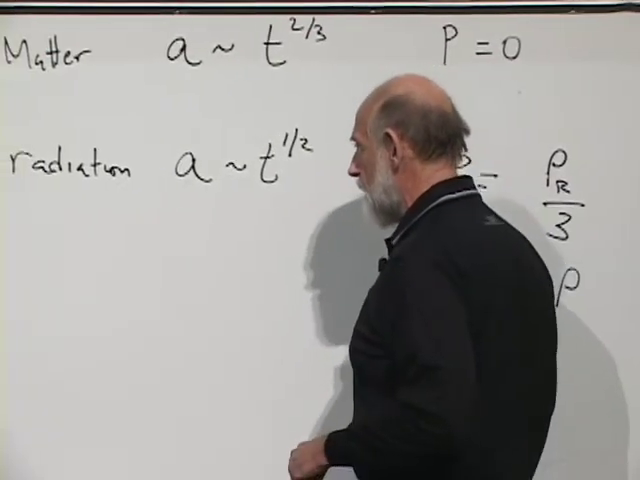
\includegraphics[width=0.74\textwidth]{lecture_04_figure_04.png}
\caption{物質與輻射：\(a\sim t^{2/3}\)、\(P=0\)；以及 \(a\sim t^{1/2}\)、\(P=\rho/3\)。}
\end{figure}

黑板上的摘要是
\begin{align}
\text{matter:}\qquad & a(t)\sim t^{2/3}, \qquad P=0,\\
\text{radiation:}\qquad & a(t)\sim t^{1/2}, \qquad P=\frac{\rho}{3}.
\end{align}

\begin{classroomqa}
\lecturetimestamp{00:54:27}
\audiencequestion{在膨脹的宇宙中，粒子不是實際上正在彼此遠離嗎？}
\lecturerresponse{是的，但壓力的論證是針對無窮小的共動盒子進行。在這個局部尺度上，熱力學推理仍然成立。}
\end{classroomqa}

\section{狀態方程}

我們假設壓力與能量密度成正比，
\begin{equation}
P=w\rho .
\end{equation}
黑板上用 \(\omega\) 表示同一個參數。兩種基本情況分別是
\begin{equation}
w=0 \quad \text{for cold matter},
\qquad
w=\frac{1}{3} \quad \text{for radiation}.
\end{equation}

也可能有介於 \(0\) 和 \(1/3\) 之間的值，代表既非完全冷態、也非完全相對論性的物質。這裡提到的例子是溫暖暗物質。

\begin{figure}
\centering
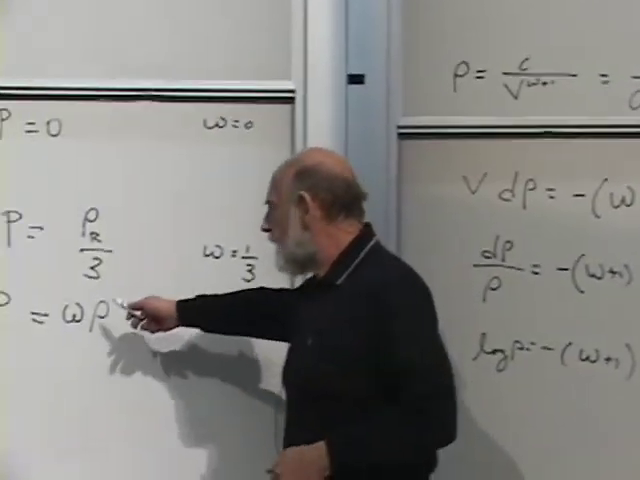
\includegraphics[width=0.74\textwidth]{lecture_04_figure_05.png}
\caption{狀態方程 \(P=\omega\rho\) 與密度標度的推導。}
\end{figure}

接下來要問的是，\(w\) 是否決定 \(\rho\) 對 \(a\) 的依賴關係。答案可由熱力學恆等式推得。

取一個體積為 \(V\) 的盒子。如果盒中物質施加壓力 \(P\)，那麼盒子膨脹 \(dV\) 時，對盒壁所做的功為
\begin{equation}
dE=-P\,dV.
\end{equation}
現在將能量寫成
\begin{equation}
E=\rho V.
\end{equation}
其微分為
\begin{equation}
dE=\rho\,dV+V\,d\rho .
\end{equation}
令兩個表示式相等，得到
\begin{equation}
\rho\,dV+V\,d\rho=-P\,dV,
\end{equation}
也就是
\begin{equation}
V\,d\rho=-(\rho+P)\,dV.
\end{equation}
利用 \(P=w\rho\)，可得
\begin{equation}
V\,d\rho=-(1+w)\rho\,dV.
\end{equation}
兩邊除以 \(\rho V\)：
\begin{equation}
\frac{d\rho}{\rho}=-(1+w)\frac{dV}{V}.
\end{equation}
積分後，
\begin{equation}
\rho \propto V^{-(1+w)}.
\end{equation}
對共動的宇宙學盒子而言，
\begin{equation}
V\propto a^3,
\end{equation}
因此
\begin{equation}
\rho \propto a^{-3(1+w)}.
\end{equation}

立刻就能得到前面討論的情況：
\begin{align}
w=0 &\Longrightarrow \rho \propto a^{-3},\\
w=\frac{1}{3} &\Longrightarrow \rho \propto a^{-4}.
\end{align}

這就是 \(w\) 重要的原因。知道 \(\rho(a)\) 之後，就能將它代回弗里德曼方程。接著設 \(a\sim t^\alpha\) 為冪律形式，便可求出該狀態方程下宇宙的膨脹方式。

\section{真空能與負壓力}

有一種特殊情況有所不同：
\begin{equation}
w=-1.
\end{equation}
於是
\begin{equation}
1+w=0,
\end{equation}
指數項便為零，因此
\begin{equation}
\rho=\rho_0=\text{constant}.
\end{equation}
相應的壓力為
\begin{equation}
P=-\rho .
\end{equation}

負壓力本身並不神秘。正壓力會向外推盒壁；負壓力則向內拉，也就是張力。拉緊的橡皮筋就是日常生活中的例子：它儲存正能量，卻會把兩端拉在一起。

把常數密度 \(\rho_0\) 代入弗里德曼方程：
\begin{equation}
\left(\frac{\dot a}{a}\right)^2=\frac{8\pi G}{3}\rho_0.
\end{equation}
右側只是常數，因此
\begin{equation}
\frac{\dot a}{a}=\sqrt{\frac{8\pi G}{3}\rho_0}.
\end{equation}
這是哈伯參數確實為常數的特殊情況。方程可以寫成
\begin{equation}
\dot a=\sqrt{\frac{8\pi G}{3}\rho_0}\,a,
\end{equation}
其解為
\begin{equation}
a(t)\propto \exp\!\left(\sqrt{\frac{8\pi G}{3}\rho_0}\,t\right).
\end{equation}

這就是指數膨脹。相關的時間尺度是 \(e\) 倍增時間，而不是加倍時間；這裡採用的粗略估計指出，它的量級約等於宇宙年齡。除歷史上採用的數值慣例外，真空能與宇宙學常數指的是同一種物理成分。

\begin{classroomqa}
\lecturetimestamp{01:27:16}
\audiencequestion{如果真空能驅動指數膨脹，最後所有東西不都會被撕裂嗎？}
\lecturerresponse{不一定。束縛系統可以抵抗膨脹。星系、太陽系或原子不一定會被撕裂；但夠大且稀疏的結構會隨宇宙膨脹，最後彼此分離。}
\end{classroomqa}

\begin{classroomqa}
\lecturetimestamp{01:31:43}
\audiencequestion{對弗里德曼方程開平方時，負號有什麼值得注意之處嗎？}
\lecturerresponse{有。開平方後會得到兩個分支：一個是膨脹解，另一個是時間反演後的收縮解。方程本身容許這兩種解。}
\end{classroomqa}

\section{三個時代與觀測到的膨脹歷史}

三種組分都存在，而且密度隨尺度因子的變化方式各不相同：
\begin{equation}
\begin{aligned}
\rho_{\text{radiation}}&\propto a^{-4},\\
\rho_{\text{matter}}&\propto a^{-3},\\
\rho_0&=\text{constant}.
\end{aligned}
\end{equation}
這立刻導出三個時代。

當 \(a\) 極小時，輻射佔主導。之後由物質佔主導。當 \(a\) 足夠大時，真空能佔主導。相應的膨脹定律為
\begin{equation}
a(t)\sim t^{1/2},
\qquad
a(t)\sim t^{2/3},
\qquad
a(t)\sim e^{Ht}.
\end{equation}

這裡引用的粗略時間如下：大約經過 \(10^4\) 年後，輻射主導轉為物質主導。大約經過 \(10^5\) 年後，宇宙才變得透明。物質主導轉為加速膨脹則晚得多，發生在數十億年後；依此處採用的數量級估算，約在宇宙歷史的中點。

我們如何推斷這段歷史？我們看不到未來，但看得到過去。觀測距離越遠，就越是在看更早的時刻。觀測遙遠星系、測量其運動與距離的關係，再重建哈伯參數隨回溯時間的變化，就能重建尺度因子的時間演變。輻射主導時代太早，無法透過一般星系天文觀測直接看見；但從重建曲線中，可以看見物質主導時代以及轉入真空能主導的過程。

\section{遙遠未來的最後散射}

未來的微波天空與星系越過視界而消失，是兩回事。我們在較晚時刻看到的輻射來自更遠處的物質，因此我們看到的是更深、更冷的宇宙，而不是看著同一批原子單純地退行遠去。

\begin{classroomqa}
\lecturetimestamp{01:48:07}
\audiencequestion{如果最後散射面逐漸隱沒在視界中，這和星系移到視界之外是同一回事嗎？}
\lecturerresponse{不是。較晚時刻看到的輻射，並非來自我們現在看到的同一批原子，而是來自更遠處的原子。這就像我們越看越深入宇宙，同時看到的輻射也越來越冷。}
\end{classroomqa}

\section{曲率、大擠壓圖像與晚期視界}

到目前為止，曲率項都省略了。把它加回來，得到
\begin{equation}
\left(\frac{\dot a}{a}\right)^2
=
\frac{8\pi G}{3}\rho
-
\frac{K}{a^2}.
\end{equation}
這一項的數值看起來很小，但在概念上很重要。用較早期的牛頓力學語言來說，它區分總能量為正、為零和為負的情況；用相對論的語言來說，它區分不同的空間幾何。

過去人們還沒有認真看待真空能時，常設想一個由物質主導、膨脹最終會反轉的宇宙。這就是舊有的大擠壓圖像：宇宙從大爆炸開始膨脹，之後再度收縮。這套數學仍然成立，但看來已不適用於我們的宇宙。

\begin{classroomqa}
\lecturetimestamp{01:53:51}
\audiencequestion{這種真空能和量子真空能有關嗎？}
\lecturerresponse{有關，至少一般相信兩者有關。}
\end{classroomqa}

目前宇宙的組成大致為
\begin{equation}
\frac{\rho_0}{\rho_{\text{total}}}\sim 0.7,
\qquad
\frac{\rho_{\text{matter}}}{\rho_{\text{total}}}\sim 0.3.
\end{equation}
在物質組分中，發光物質約佔總量的 \(0.05\)，暗物質約佔 \(0.25\)。目前輻射所佔的比例可以忽略。暗物質和發光物質的密度以相同方式隨尺度因子變化，因此即使物質、輻射和真空能的相對含量隨時代改變，兩者的比例仍固定。

在真空能主導的極限下，
\begin{equation}
H=\sqrt{\frac{8\pi G}{3}\rho_0}.
\end{equation}
於是哈伯定律變為
\begin{equation}
v=Hd.
\end{equation}
視界定義為 \(v=1\)，所以其距離為
\begin{equation}
d_H=\frac{1}{H}
=
\frac{1}{\sqrt{8\pi G\rho_0/3}}.
\end{equation}
這裡給出的粗略數值約為 \(10\) 至 \(12\) 十億光年。

重要的是晚期的行為。膨脹一旦進入指數形式，視界距離就會固定。星系仍會越過視界，並因紅移愈來愈大而消失。微波背景也會逐漸紅移到不可見。在遙遠未來，只有附近受引力束縛的結構仍可觀測，宇宙看起來會像一座孤島。

\section{從最後散射面測量幾何}

最後，可以透過最後散射面來檢驗幾何。假設我們已知到該表面的距離，也能在那裡辨認出一個物理大小已知得夠準確的團塊。接著就能把它的大小和距離與觀測到的角大小作比較。

在平坦空間中，角度符合歐幾里得幾何。在正曲率空間中，物體看起來會較大；在負曲率空間中則會較小。這就像一般測量：對已知距離、已知大小的物體測量角度，再與歐幾里得幾何的預測比較。

\begin{classroomqa}
\lecturetimestamp{02:08:09}
\audiencequestion{有什麼遠方物體的大小是我們已知的？}
\lecturerresponse{微波背景中最大的團塊。我們認為，從它們演化所需的時間以及聲速，可以推知其大小。}
\end{classroomqa}

這裡考慮的是微波背景中最大的團塊。觀測到的角大小與歐幾里得幾何的預測相符，差異在百分之幾以內。根據這項結果，空間看來是平坦的。

\section{測得的 \(w\) 與最後一個問題}

現在可以看出 \(w\) 在觀測上的重要性。如果天文學家報告說 \(w\) 非常接近 \(-1\)，他們的意思是真空能組分幾乎是常數。這正是這裡要指出的重點。

這並不表示廣義相對論迫使 \(w\) 恰好等於 \(-1\)。這裡談的是經驗結果。講座簡短提到，原則上不能排除更激進的可能性；但有充分理由相信，真空能近乎為常數的情況確實成立。

\begin{classroomqa}
\lecturetimestamp{02:11:04}
\audiencequestion{在計算物質和輻射的密度時，我們是否先假設能量保持不變，再調整尺度因子來求出公式？如果前兩種情況都是如此，那麼真空能的情況又如何？在那種情況下，密度保持不變。}
\lecturerresponse{不，我沒有假設能量保持不變。我們用的是能量變化量 \(-P\,dV\)。對於一個假想的共動盒子，它隨著宇宙膨脹而移動，膨脹時會對盒壁做功，這就解釋了能量的變化。真空能的情況引出了另一個問題；最後要補充的是，在宇宙學中談能量守恆意義不大，因為宇宙的總能量為零。}
\end{classroomqa}